\chapter{Struttura di un log HTTP e Machine Learning}
\section{Il protocollo HTTP in generale }
In telecomunicazioni ed informatica \emph{l’HyperText Transfer Protocol} è un protocollo di tipo applicativo usato come principale sistema per la trasmissione di informazioni su internet. La prima versione del protocollo, la HTTP/0.9, venne implementata da Tim Berners-Lee, allora studioso del CERN di Ginevra ed aveva come fine ultimo la condivisione di informazioni tra la comunità scientifica \parencite{berners1989}

Successivamente vennero rilasciate versioni che rispondevano, man mano, alle esigenze che si manifestavano.

In breve:
\begin{itemize}
    \item HTTP/1.0, la prima versione effettivamente disponibile del protocollo ed implementata dallo stesso Berners-Lee \parencite{rfc1945}
    \item HTTP/1.1, presentato come RFC 2068 \parencite{rfc2068} ed aggiornato come descritto nel RFC 2616 \parencite{rfc2616}
    \item HTTP/2 e HTTP/3 pubblicate rispettivamente nelle RFC 7540 \parencite{rfc7540}  e RFC 9114 \parencite{rfc9114}
\end{itemize}

Il protocollo HTTP, come definito nell’RFC9110, lavora al livello più alto dello standard OSI \parencite{rfc9110}  con un tipo di architettura definito client/server dove il client esegue una richiesta ed il server restituisce la risposta mandata da un altro host. Nell’uso quotidiano il client corrisponde al browser mentre il server (sia quest’ultimo virtuale o fisico) è la macchina su cui risiede il sito web.

\section{Log HTTP, definizione e struttura }
Pur non esistendo una definizione formale di \emph{log HTTP} all’interno delle specifiche del protocollo, con tale espressione si fa riferimento al file generato dal server web che registra in maniera strutturata le richieste ricevute e le relative risposte fornite. Il log rappresenta dunque una traccia persistente dell’attività del server e costituisce uno strumento fondamentale per il monitoraggio della sicurezza, la diagnosi di errori applicativi, l’analisi delle performance e lo studio del traffico.

Il primo formato strutturato per i log web è il Common Log Format (CLF), sviluppato nell’ambito del progetto NCSA HTTPd \parencite{w3clogging}, presso il National Center for Supercomputing Applications. Si riporta di seguito estratto dell’archivio del World Wide Web Consortium che descrive la struttura del CLF (si veda la figura \ref{fig:clf}).

\begin{figure}[H]
    \centering
    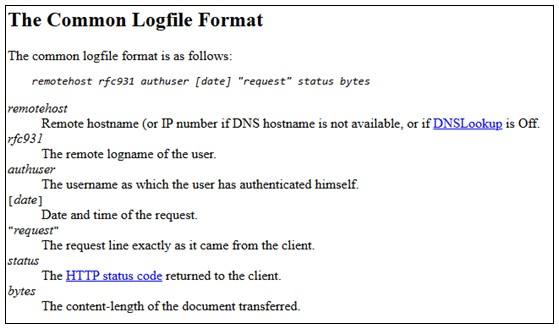
\includegraphics[width=\textwidth]{Immagini/CLF.jpg}
    \caption{W3C - Common Logfile Format}
    \label{fig:clf}
\end{figure}

Un esempio concreto risulta così strutturato:

\begin{lstlisting}[style=LogStyle]
127.0.0.1 - frank [10/Oct/2000:13:55:36 -0700] "GET /index.html HTTP/1.0" 200 2326
\end{lstlisting}

Ogni riga risulta essere una singola richiesta HTTP e contiene informazioni relative al client, al tipo di richiesta al codice di stato restituito ed infine la dimensione della risposta.

\section{Log HTTP, Datamodel per il caso studio}

Per il caso di studio oggetto della presente tesi, ci si avvale di un dataset precostruito e pubblicamente disponibile, scaricato dalla piattaforma Zenodo \parencite{zenodoLog} , repository open-access per la condivisione di dati di ricerca.

Il dataset selezionato contiene log HTTP provenienti da un ambiente reale e già sottoposti a un processo di anonimizzazione, al fine di garantire la tutela di eventuali informazioni sensibili. Tale scelta consente di operare su dati realistici, mantenendo al contempo conformità ai principi di protezione dei dati.

Di seguito si riporta un estratto esemplificativo di una riga di log convertito in formato JSON tratta dal dataset:

\begin{lstlisting}[style=LogStyle]
{
    "referrer":"http://search.lib.auth.gr/Record/xxxxx",
    "request":"search.lib.auth.gr:80 66.249.34457 - - [01/Mar/2018:00:00:01 +0200] GET /AJAX/xxxxxxxx
    HTTP/1.1 200 491 http://search.lib.auth.gr/Record/xxxxx Mozilla/5.0 (compatible; Googlebot/2.1; +http://www.google.com/bot.html)",
    "method":"GET",
    "resource":"/AJAX/xxxxxx",
    "bytes":"491",
    "response":"200",
    "ip":"66.249.34457",
    "useragent": "Mozilla/5.0 (compatible; Googlebot/2.1; +http://www.google.com/bot.html)",
    "timestamp": "2018-02-28T22:00:01.000Z",
    "log_id": "-7RfsmoBCue8G08E1FyY",
}
\end{lstlisting}

\begin{itemize}
    \item \emph{Referrer}: URL della pagina da cui proviene la richiesta.
    \item \emph{Request}: Stringa completa del log HTTP.
    \item \emph{Method}: Tipologia della richiesta (GET,POST,ecc).
    \item \emph{Resource}: Path richiesto sul server.
    \item \emph{Bytes}: Numero di bytes restituiti nella response.
    \item \emph{Response}: Tipo di HTTP Status codice \begin{itemize}
              \item 2xx - Ok.
              \item 3xx - Redirect.
              \item 4xx - Not found.
              \item 5xx - Server error.
          \end{itemize}
    \item \emph{Ip}: Indirizzo IP del client che ha fatto la richiesta
    \item \emph{Useragent}: Informazioni sul browser e sistema operativo oppure bot che ha effettuato la richiesta.
    \item \emph{Timestamp}: Formato ISO 8601(YYYY-MM-DDThh:mm:ssZ), rappresenta date e ore in modo standardizzato. Utilizza la lettera “T” per separare la data dall’ora e la Z per UTC \parencite{iso8601}.
    \item \emph{Log Id}: Chiave univoca del file JSON, non ha significato semantico lato HTTP.

\end{itemize}

Come si può intuire dal formato e dai campi del datamodel preso in esame e come accennato in precedenza, quest’ultimo risulta già sottoposto ad un preprocesso di parsing.

Per valutare la fattibilità in scenari reali, è stato convalidato che gli stessi campi strutturati possono essere estratti dalle righe di registro non elaborate utilizzando l'analisi deterministica che tuttavia esula dal fine ultimo di questa tesi.

\section{Intelligenza artificiale e machine learning}
Allo stato attuale dell’evoluzione di tutto ciò che concerne gli ambiti IT, concetti come Intelligenza Artificiale e \emph{Machine Learning} rappresentano le innovazioni più rilevanti e diffuse essendo, queste ultime, capaci di incidere significativamente sugli aspetti produttivi.

L’intelligenza artificiale viene definita come “... l’abilità di una macchina di mostrare capacità umane quali il ragionamento, l’apprendimento, la pianificazione e la creatività; tali caratteristiche consentono all’IA la comprensione del proprio ambiente, l’elaborazione di ciò che viene percepito e l’individuazione di soluzioni per un obiettivo specifico.” \parencite{aida2021parlamento}

Questa simulazione del ragionamento umano è consentita dall’analisi e dall’elaborazione dei \emph{Big Data}, enormi quantità di dati la cui interpretazione richiede tecnologie e metodi analitici specifici \parencite{demauro2016bigdata}.

Nell’ambito delle intelligenze artificiali moderne (e quelle prese in esame come oggetto di questa tesi) l’analisi predittiva e quella prescrittiva assumono una importanza cruciale in quanto, la prima, si avvale della capacità di apprendere e identificare pattern nei dati e quindi di anticiparli. La seconda, fornisce indicazioni per orientare le successive azioni sulla base di quanto appreso \parencite{hullermeier2021prescriptive}.
Il machine learning (ML) è un tipo di intelligenza artificiale che consente al computer senza essere stato esplicitamente programmato.
Quest’ultimo recupera informazioni da più o meno grandi set di dati ed utilizza i pattern in essi contenuti al fine di migliorarne la comprensione \parencite{sharifani2023machine}. La metodologia avanzata di ML prevede che gli algoritmi apprendano per inferenza, senza supervisione di un programmatore e, oltre ad apprendere e ad auto adattarsi, sono in grado di comprendere e rilevare alcuni schemi che l’essere umano da solo non sarebbe in grado di riconoscere. Un esempio concreto alla portata di tutti si vive nelle piattaforme di tipo social o streaming, dove i contenuti proposti dalla piattaforma stessa sono basati sulle visualizzazioni, ricerche ed interazioni di contenuti precedentemente avvenute.

\section{ML, Isolation Forest per il rilevamento di anomalie}
Isolation Forest è un algoritmo di anomaly detection non supervisionato progettato per individuare osservazioni anomale all’interno di un dataset. L’approccio si basa sul principio di isolamento delle istanze anomale invece che sulla modellazione esplicita del comportamento normale dei dati.

L’algoritmo è stato introdotto da Fei Tony Liu, Kai Ming Ting e Zhi-Hua Zhou nell’articolo “Isolation Forest”, presentato alla conferenza IEEE International Conference on Data Mining (ICDM) nel 2008 \parencite{liu2008isolation}. L’idea centrale dell’algoritmo è che le anomalie sono generalmente rare e significativamente diverse rispetto alla maggior parte dei dati osservati \parencite{liu2012isolationbased}. Di conseguenza, tali istanze risultano più facili da isolare attraverso partizioni casuali dello spazio delle feature.

A differenza di molti metodi tradizionali di rilevamento delle anomalie, che costruiscono un modello del comportamento normale dei dati e identificano come anomalie le deviazioni da tale modello, Isolation Forest mira direttamente a isolare i punti anomali. Questa caratteristica rende l’algoritmo particolarmente efficiente dal punto di vista computazionale e facilmente scalabile anche su dataset di grandi dimensioni \parencite{liu2012isolationbased}.

Un ulteriore vantaggio è rappresentato dalla scalabilità in presenza di dataset ad alta dimensionalità. Diversamente da molti metodi basati su distanze o densità (come \emph{k-Nearest Neighbors o Local Outlier Factor}), Isolation Forest utilizza suddivisioni casuali su singole feature, riducendo l’impatto della cosiddetta \emph{curse of dimensionality} \parencite{zimek2012survey}. Questa proprietà rende l’algoritmo adatto all’analisi di dati complessi e con numerose variabili.

Dal punto di vista computazionale, Isolation Forest risulta particolarmente efficiente. L’algoritmo utilizza una strategia di sub-sampling dei dati e costruisce alberi molto leggeri, con una complessità temporale approssimativamente lineare rispetto al numero di osservazioni. Inoltre, richiede una quantità limitata di memoria \parencite{liu2012isolationbased}, caratteristica che lo rende adatto all’analisi di grandi volumi di dati, come nel caso dei log HTTP generati da sistemi web.

Infine, l’algoritmo non assume specifiche distribuzioni statistiche per le feature del dataset. Questa assenza di ipotesi restrittive consente di applicarlo efficacemente anche a dati eterogenei e con distribuzioni irregolari, situazione frequente nei contesti reali di analisi dei log \parencite{chandola2009anomaly}.
Nel contesto dell’analisi dei log HTTP, queste caratteristiche rendono Isolation Forest una scelta particolarmente adatta per individuare richieste potenzialmente sospette o anomale, anche in assenza di informazioni preliminari sulle tipologie di attacco o di comportamento anomalo.

\section{Isolation Forest, principi di funzionamento}
Il funzionamento di Isolation Forest si basa sulla costruzione di una collezione di alberi binari chiamati Isolation Trees (iTree)\parencite{liu2008isolation}. Ogni albero viene costruito selezionando casualmente un sottoinsieme dei dati e applicando, a ogni nodo, due scelte casuali:

\begin{itemize}
    \item la selezione di una feature;
    \item la selezione di una soglia di split compresa tra il valore minimo e massimo della feature nel sottoinsieme corrente.
\end{itemize}
Attraverso queste suddivisioni casuali, lo spazio delle feature viene progressivamente partizionato fino a isolare le singole osservazioni.
Il principio fondamentale dell’algoritmo è che le anomalie, essendo rare e distanti dalla massa dei dati, tendono a essere isolate con un numero ridotto di suddivisioni. In termini di struttura dell’albero, questo significa che tali istanze raggiungono una foglia dopo un numero relativamente piccolo di livelli. Al contrario, i punti appartenenti a regioni dense del dataset richiedono un numero maggiore di suddivisioni per essere isolati, generando quindi cammini più lunghi all’interno dell’albero \parencite{liu2008isolation}.

Per ogni osservazione (x), viene calcolata la lunghezza media del cammino (E(h(x))) attraverso tutti gli alberi della foresta. Tale valore viene successivamente normalizzato per ottenere un punteggio di anomalia (\emph{anomaly score}). Una formulazione comune del punteggio è la seguente:
\begin{equation}
    s(x) = 2^{-\frac{E(h(x))}{c(n)}}
    \label{eq:anomaly_score}
\end{equation}

dove (c(n)) rappresenta una costante di normalizzazione dipendente dalla dimensione del campione (n) \parencite{liu2008isolation}.

Interpretando questo punteggio:
\begin{itemize}
    \item valori di (s(x)) prossimi a 1 indicano che l’istanza ha un cammino medio breve e quindi è probabilmente un’anomalia;
    \item valori di (s(x)) prossimi a 0 indicano invece un comportamento coerente con quello della maggioranza dei dati.
\end{itemize}

Infine, per classificare le osservazioni come normali o anomale è possibile definire una soglia sul punteggio di anomalia oppure specificare un parametro di \emph{contamination}, che rappresenta la percentuale attesa di anomalie nel dataset. In questo modo il modello può identificare automaticamente richieste HTTP sospette o comportamenti anomali all’interno dei log analizzati \parencite{scikit-learn}.

Questo approccio consente quindi di effettuare un rilevamento automatico delle anomalie in modo efficiente e scalabile.